\documentclass[11pt]{article}
\usepackage[margin=1in]{geometry}
\usepackage{amsmath,amssymb,amsthm}
\usepackage{graphicx,float}
\usepackage{lmodern}
\usepackage[T1]{fontenc}
\usepackage{xcolor,framed,booktabs,microtype,array}
\usepackage[colorlinks=true,linkcolor=blue!60!black,urlcolor=blue!60!black]{hyperref}

\definecolor{shadecolor}{RGB}{240,244,250}
\definecolor{warncolor}{RGB}{253,242,235}
\newenvironment{keyidea}{\begin{shaded}\noindent\textbf{Key idea.} }{\end{shaded}}
\newenvironment{pitfall}{\colorlet{shadecolor}{warncolor}\begin{shaded}\noindent\textbf{Common pitfall.} }{\end{shaded}}
\newenvironment{template}{\begin{framed}\noindent\textbf{Recipe.} }{\end{framed}}

\newcommand{\R}{\mathbb{R}}
\newcommand{\T}{^{\mathsf T}}
\newcommand{\ones}{\mathbf{1}}

\theoremstyle{definition}
\newtheorem{definition}{Definition}[section]
\theoremstyle{plain}
\newtheorem{theorem}[definition]{Theorem}
\newtheorem{proposition}[definition]{Proposition}
\theoremstyle{remark}
\newtheorem{example}[definition]{Example}
\newtheorem{exercise}{Self-test}

\title{LP Duality, Complementary Slackness,\\ and Theorems of the Alternative\\ \large A study guide for the material of Homework 3}
\author{Optimization (Caramanis \& Sanghavi) --- companion notes}
\date{\today}

\begin{document}
\maketitle
\tableofcontents
\bigskip

\section{Why duality}
Every linear program comes with a twin, its \emph{dual}. The dual answers a question the primal cannot answer by itself: \emph{how do I know a proposed solution is optimal?} A feasible $x$ proves ``the optimum is at most $c\T x$''; a dual-feasible $p$ proves ``the optimum is at least $p\T b$.'' When the two numbers meet, optimality is \emph{certified}. The same mechanism certifies infeasibility (Farkas' lemma) and explains which constraints matter at the optimum (complementary slackness). Homework~3 exercises the three core skills:
\begin{itemize}
\item mechanically forming a dual, with every sign right (Problem 1);
\item converting a logical statement about linear inequalities into an LP and reading off the alternative from its dual (Problem 2);
\item exploiting the \emph{structure} of dual solutions, namely sparsity of vertices and complementary slackness (Problem 3).
\end{itemize}

\section{Forming the dual}
\subsection{The dictionary}
For a \textbf{minimisation} primal with cost $c$, constraint matrix $A$ (rows $a_i\T$, columns $A_j$) and right-hand side $b$:
\begin{center}\renewcommand{\arraystretch}{1.2}
\begin{tabular}{@{}l@{\qquad}l@{\qquad\qquad}l@{\qquad}l@{}}\toprule
\multicolumn{2}{c}{\textbf{Primal:} $\min\ c\T x$} & \multicolumn{2}{c}{\textbf{Dual:} $\max\ p\T b$}\\ \midrule
$i$-th constraint & $a_i\T x\ge b_i$ & $i$-th variable & $p_i\ge0$\\
 & $a_i\T x\le b_i$ & & $p_i\le0$\\
 & $a_i\T x= b_i$ & & $p_i$ free\\[3pt]
$j$-th variable & $x_j\ge0$ & $j$-th constraint & $p\T A_j\le c_j$\\
 & $x_j\le0$ & & $p\T A_j\ge c_j$\\
 & $x_j$ free & & $p\T A_j= c_j$\\ \bottomrule
\end{tabular}\end{center}
One dual variable per primal constraint; one dual constraint per primal variable. For a \textbf{maximisation} primal, read the table right-to-left.

\emph{Mnemonic (``natural $\leftrightarrow$ nonnegative'').} In a min problem the natural constraint direction is $\ge$; in a max problem it is $\le$. A natural constraint gives a nonnegative multiplier, an unnatural one a nonpositive multiplier, an equality a free one. Symmetrically, a nonnegative variable gives a natural dual constraint, a nonpositive variable an unnatural one, a free variable an equality.

\subsection{Where the dictionary comes from: the Lagrangian}
Relax the general constraints with prices $p$ and define
\[
g(p)=\min_{x\ \text{obeying its sign constraints}}\ \Big[c\T x+p\T(b-Ax)\Big]=p\T b+\min_x\ \sum_j\big(c_j-p\T A_j\big)x_j .
\]
\begin{enumerate}
\item \textbf{Signs of $p$} are chosen so that the penalty $p\T(b-Ax)$ is $\le0$ at every feasible $x$. Then $g(p)\le c\T x$ for all feasible $x$: every such $p$ yields a lower bound.
\item \textbf{Dual constraints} are exactly the conditions for the inner minimum to be finite (it is then $0$). If $x_j\ge0$ we need $c_j-p\T A_j\ge0$; if $x_j\le0$, $\le0$; if $x_j$ is free, $=0$.
\item The dual is ``find the best lower bound'': $\max_p g(p)$.
\end{enumerate}
If you forget the table, this three-line derivation rebuilds it, and it is the same construction that defines the dual of a general convex program later in the course.

\subsection{The standard pairs worth memorising}
\begin{center}\renewcommand{\arraystretch}{1.25}
\begin{tabular}{@{}ll@{}}\toprule
Primal & Dual\\ \midrule
$\min c\T x$ \ s.t.\ $Ax=b,\ x\ge0$ \ (standard form) & $\max p\T b$ \ s.t.\ $A\T p\le c$\\
$\min c\T x$ \ s.t.\ $Ax\ge b,\ x\ge0$ \ (symmetric form) & $\max p\T b$ \ s.t.\ $A\T p\le c,\ p\ge0$\\
$\min c\T x$ \ s.t.\ $Ax\ge b$ & $\max p\T b$ \ s.t.\ $A\T p=c,\ p\ge0$\\
$\max c\T x$ \ s.t.\ $Ax\le b,\ x\ge0$ & $\min b\T y$ \ s.t.\ $A\T y\ge c,\ y\ge0$\\ \bottomrule
\end{tabular}\end{center}

\begin{example}[HW3 Problem 1]
$\min x_1-x_2$ with rows of type $\le,\ \ge,\ =$ and variables $x_1\le0$, $x_2,x_3\ge0$, $x_4$ free. Rows give $p_1\le0$, $p_2\ge0$, $p_3$ free. Columns give, in order, a ``$\ge c_1$'' constraint, two ``$\le c_j$'' constraints and one equality. The objective is $b\T p=3p_2+6p_3$. For this instance the dual is infeasible and the primal unbounded, a reminder that ``compute the dual'' and ``the dual has a solution'' are different questions.
\end{example}

\begin{pitfall}
\begin{itemize}
\item \textbf{A variable with no stated sign is free}, and produces an \emph{equality} in the dual. (In HW3 P1, $x_4$.)
\item \textbf{The dictionary depends on min vs.\ max.} Applying the min-table to a max problem flips every sign. When unsure, convert to a min problem first, or redo the Lagrangian argument.
\item \textbf{Do not convert to standard form first} unless asked: it works (equivalent primals have equivalent duals) but doubles the bookkeeping and the chance of error.
\item \textbf{Check dimensions}: $p\in\R^{\#\text{constraints}}$, and there are $\#\text{variables}$ dual constraints. Sign restrictions on $x$ are \emph{not} counted as constraints here.
\end{itemize}
\end{pitfall}

\begin{proposition}
The dual of the dual is the primal. Equivalent formulations of the primal (slack variables, splitting $x=x^+-x^-$, negating rows) have equivalent duals.
\end{proposition}

\section{Weak and strong duality}
\begin{theorem}[Weak duality]
If $x$ is primal feasible (min problem) and $p$ is dual feasible, then $p\T b\le c\T x$.
\end{theorem}
\begin{proof}
$c\T x-p\T b=\sum_j(c_j-p\T A_j)x_j+\sum_ip_i(a_i\T x-b_i)$, and the dictionary was built so that every term in both sums is $\ge0$.
\end{proof}
\begin{figure}[H]\centering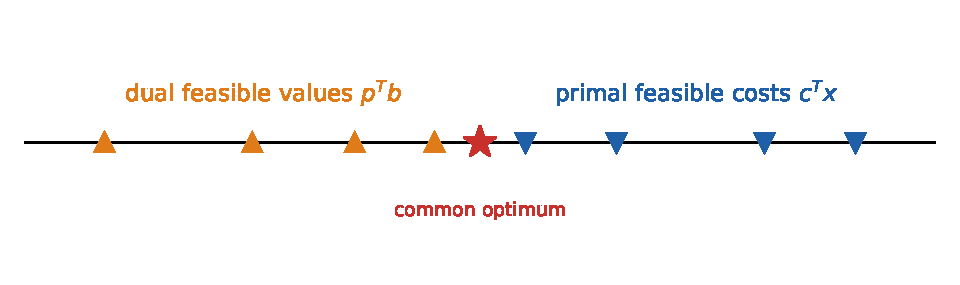
\includegraphics[width=.62\textwidth]{figures/g_weak_duality.pdf}\end{figure}
Immediate consequences: (a) primal unbounded $\Rightarrow$ dual infeasible; (b) dual unbounded $\Rightarrow$ primal infeasible; (c) if $c\T x=p\T b$ for a feasible pair, both are optimal.

\begin{theorem}[Strong duality]
If an LP has an optimal solution, so does its dual, and the optimal values are equal.
\end{theorem}
For LPs there is no constraint qualification and no duality gap: feasibility plus boundedness is enough. (For general convex programs one needs a condition such as Slater's.)

\paragraph{The possibilities table.}
\begin{center}\renewcommand{\arraystretch}{1.2}
\begin{tabular}{@{}lccc@{}}\toprule
 & Dual: finite optimum & Dual: unbounded & Dual: infeasible\\ \midrule
Primal: finite optimum & \textbf{possible} (equal values) & impossible & impossible\\
Primal: unbounded & impossible & impossible & \textbf{possible}\\
Primal: infeasible & impossible & \textbf{possible} & \textbf{possible}\\ \bottomrule
\end{tabular}\end{center}
HW3 P1 lives in the middle-right cell. The bottom-right cell is real: $\min x_1+2x_2$ s.t.\ $x_1+x_2=1$, $2x_1+2x_2=3$ is infeasible, and its dual $\max p_1+3p_2$ s.t.\ $p_1+2p_2=1$, $p_1+2p_2=2$ is infeasible too.

\begin{pitfall}
``Dual infeasible'' does \emph{not} imply ``primal unbounded'': the primal might be infeasible. To conclude unboundedness you must also exhibit a primal feasible point (as in P1: $x^0=(0,0,2,2)$).
\end{pitfall}

\paragraph{Interpretation.} The optimal $p_i$ is the \emph{shadow price} of constraint $i$: the rate of change of the optimal cost per unit change of $b_i$ (when the optimal basis is nondegenerate). A constraint with slack has price zero, which is the content of the next section.

\section{Complementary slackness}
\begin{theorem}[Complementary slackness]
Let $x$ be primal feasible and $p$ dual feasible. They are both optimal if and only if
\[
p_i\,(a_i\T x-b_i)=0\ \ \forall i\qquad\text{and}\qquad(c_j-p\T A_j)\,x_j=0\ \ \forall j .
\]
\end{theorem}
\begin{proof}
From the proof of weak duality, $c\T x-p\T b$ is a sum of nonnegative terms, namely exactly the products above. The gap is zero iff every term is zero, and a zero gap is equivalent to optimality of both (weak + strong duality).
\end{proof}
In words: \emph{a positive price forces a tight constraint; a slack constraint forces a zero price} (and likewise for variables versus dual constraints).

\begin{figure}[H]\centering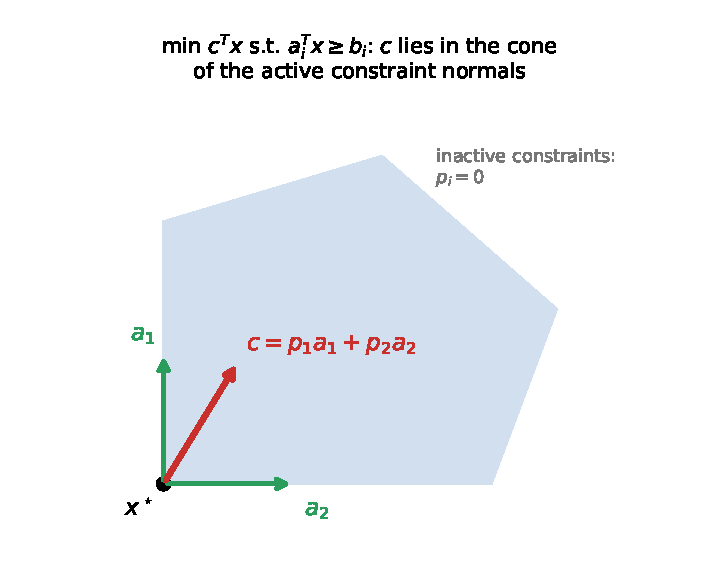
\includegraphics[width=.5\textwidth]{figures/g_comp_slack.pdf}\end{figure}
\noindent\emph{Geometry.} For $\min c\T x$ s.t.\ $a_i\T x\ge b_i$, the dual constraint is $c=\sum_ip_ia_i$ with $p\ge0$, and complementary slackness allows $p_i>0$ only on active constraints. So $x^\star$ is optimal iff $c$ lies in the cone generated by the normals of the constraints active at $x^\star$. This is the LP case of the KKT conditions.

\begin{template}
\textbf{Using complementary slackness to certify or find solutions.}
\begin{enumerate}
\item Given a candidate $x$: check primal feasibility; list the tight constraints and the nonzero variables.
\item Set $p_i=0$ for every slack constraint; impose $p\T A_j=c_j$ for every $j$ with $x_j\ne0$. Solve this (usually square) linear system.
\item Check that the resulting $p$ is dual feasible (signs and remaining constraints). If yes, $x$ and $p$ are optimal; if the system is inconsistent or $p$ infeasible (and $x$ is nondegenerate), $x$ is not optimal.
\end{enumerate}
\end{template}

\begin{example}
$\min 13x_1+10x_2+6x_3$ s.t.\ $5x_1+x_2+3x_3=8$, $3x_1+x_2=3$, $x\ge0$, candidate $x=(1,0,1)$. Dual: $\max 8p_1+3p_2$ s.t.\ $5p_1+3p_2\le13$, $p_1+p_2\le10$, $3p_1\le6$. Since $x_1,x_3>0$: $5p_1+3p_2=13$ and $3p_1=6$, so $p=(2,1)$. Check the remaining constraint: $2+1\le10$. Feasible, so both are optimal; values $13+6=19=16+3$.
\end{example}

\section{Theorems of the alternative}
A \emph{theorem of the alternative} states that exactly one of two linear systems is solvable. The second system is a \textbf{certificate}: a short proof that the first has no solution.

\begin{theorem}[Farkas' lemma]
Exactly one of the following holds:\quad (a) $\exists x\ge0$ with $Ax=b$;\qquad (b) $\exists p$ with $p\T A\ge0$ and $p\T b<0$.
\end{theorem}
\begin{proof}
\emph{Not both:} $0\le(p\T A)x=p\T b<0$ is absurd. \emph{At least one:} consider $\max 0\T x$ s.t.\ $Ax=b,\ x\ge0$, whose dual is $\min p\T b$ s.t.\ $p\T A\ge0$. The dual is feasible ($p=0$). If (a) fails the primal is infeasible, so the dual cannot have a finite optimum (strong duality would hand the primal an optimal solution); hence the dual is unbounded, giving $p$ with $p\T A\ge0$, $p\T b<0$.
\end{proof}

\begin{figure}[H]\centering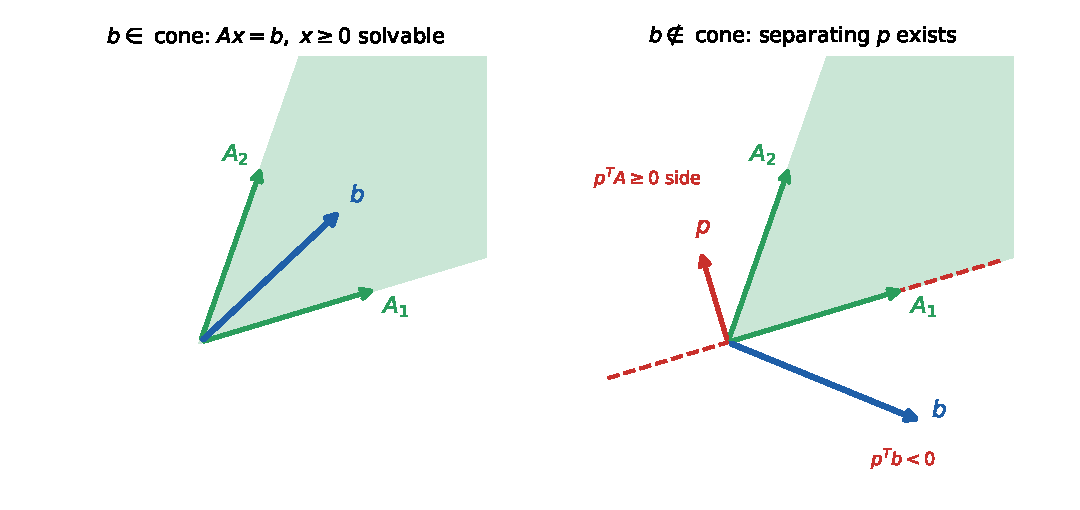
\includegraphics[width=.8\textwidth]{figures/g_farkas.pdf}\end{figure}
\noindent\emph{Geometry.} (a) says $b$ lies in the cone generated by the columns of $A$. If it does not, a hyperplane through the origin separates $b$ from that (closed, convex) cone, and its normal is $p$. Farkas' lemma is the separating hyperplane theorem for finitely generated cones.

\paragraph{The family.} All are proved the same way.
\begin{center}\renewcommand{\arraystretch}{1.25}
\begin{tabular}{@{}lll@{}}\toprule
System I & System II (certificate that I fails) & Name\\ \midrule
$Ax=b,\ x\ge0$ & $p\T A\ge0,\ p\T b<0$ & Farkas\\
$Ax\le b$ & $p\ge0,\ A\T p=0,\ b\T p<0$ & Farkas (inequality form)\\
$Ax\le b,\ x\ge0$ & $p\ge0,\ A\T p\ge0,\ b\T p<0$ & Farkas (mixed)\\
$Ax<0$ & $p\ge0,\ p\ne0,\ A\T p=0$ & Gordan\\
$Ax\ge0,\ x\ge0,\ x_1>0$ & $p\ge0,\ p\T A\le0,\ p\T A_1<0$ & HW3 Problem 2\\ \bottomrule
\end{tabular}\end{center}

\begin{template}
\textbf{Proving a theorem of the alternative.}
\begin{enumerate}
\item \emph{Easy direction (not both).} Assume both systems hold, multiply the inequalities of I by the multipliers of II and add. You should reach $0\le\dots<0$ or ``a sum of nonpositive terms is $\ge0$, so each term vanishes.''
\item \emph{Hard direction.} Encode system I as an LP: objective $0$ for a pure feasibility question, or the strict quantity as the objective (HW3 P2: $\min-x_1$ over the cone). Make sure the LP is \emph{feasible}.
\item Take the dual with the dictionary.
\item Conclude with strong duality: ``primal has an optimal solution $\Rightarrow$ dual feasible,'' or ``primal infeasible and dual feasible $\Rightarrow$ dual unbounded.'' The dual-feasible (or improving) vector is the certificate.
\item \emph{Strict inequalities.} LPs cannot express them. If the rest of the system is homogeneous, replace $p\T A_1<0$ by $p\T A_1\le-1$ and note that rescaling $p$ makes these equivalent.
\end{enumerate}
\end{template}

\begin{figure}[H]\centering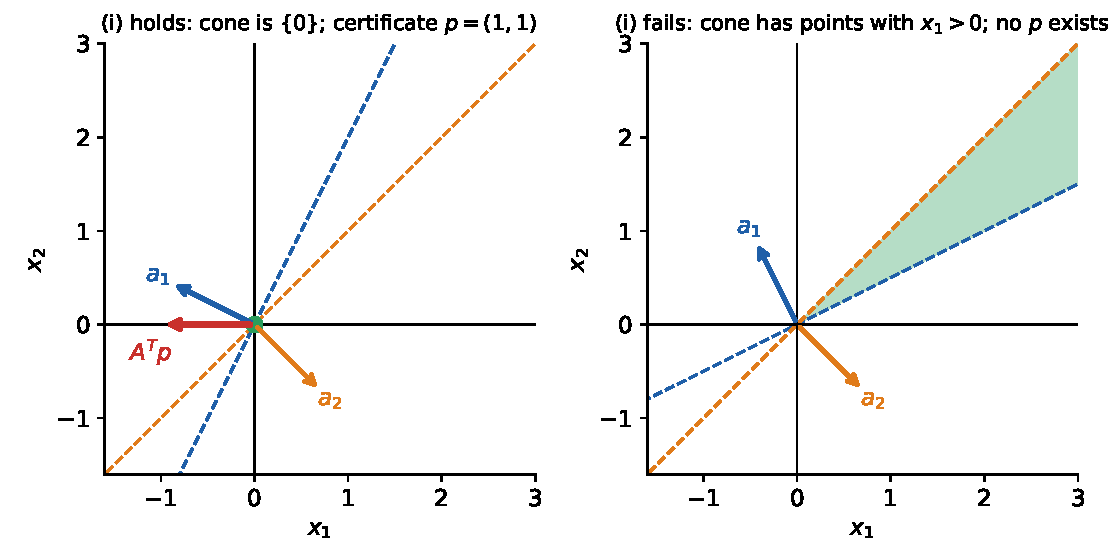
\includegraphics[width=.8\textwidth]{figures/p2_alternatives.pdf}\end{figure}
\noindent The two-panel figure shows HW3 P2 in $\R^2$. Left: the cone $\{x\ge0,Ax\ge0\}$ is $\{0\}$, and the certificate $A\T p=(-1,0)$ is a nonnegative combination of the rows that is $\le0$ with negative first entry, so ``$(A\T p)\T x\ge0$'' can hold on the orthant only when $x_1=0$. Right: the cone contains points with $x_1>0$, so no certificate exists.

\begin{pitfall}
The implication ``$Ax\ge0,\ x\ge0\Rightarrow x_1=0$'' is a statement about \emph{all} $x$; its proof via duality needs the LP to be feasible (here $x=0$ works) so that strong duality applies. Always state why the LP you wrote is feasible and bounded before invoking strong duality.
\end{pitfall}

\section{Vertices are sparse: basic solutions, Carath\'eodory, Helly}
\begin{definition}
For a standard-form polyhedron $P=\{x\in\R^N:Mx=d,\ x\ge0\}$ with $M\in\R^{k\times N}$, a \emph{basic feasible solution} (BFS) is a feasible $x$ whose positive entries correspond to linearly independent columns of $M$. BFS $=$ vertex $=$ extreme point.
\end{definition}
\begin{theorem}\leavevmode
\begin{enumerate}
\item A BFS has at most $\operatorname{rank}M\le k$ nonzero entries.
\item If $P\neq\emptyset$ it has a BFS. If the LP $\min c\T x$ over $P$ has an optimal solution, it has an optimal BFS.
\end{enumerate}
\end{theorem}
\begin{proof}[Proof idea for existence]
If the columns on the support of $x$ are dependent, take a null vector $z$ supported there, and move along $x-\theta z$ until a positive entry hits zero. Equalities are preserved, nonnegativity is preserved, the support shrinks. For the optimal version, choose the sign of $z$ so the cost does not increase. Repeat.
\end{proof}
\begin{keyidea}
\textbf{Count equality constraints to bound nonzeros.} Whenever an object is described by ``$k$ linear equations in nonnegative unknowns,'' some solution uses at most $k$ of the unknowns. Three classical faces of this one fact:
\begin{itemize}
\item \emph{Carath\'eodory:} a point in the convex hull of a set in $\R^n$ is a convex combination of at most $n+1$ of its points ($n$ equations for the point, $1$ for $\sum\lambda_i=1$).
\item \emph{HW3 P3 / Helly:} an infeasible system $Ax\le b$ in $n$ variables has an infeasible subsystem of at most $n+1$ inequalities ($n$ equations $A\T p=0$, $1$ normalisation).
\item \emph{Sparse LP solutions:} an LP with $k$ constraints needs at most $k$ nonzero variables.
\end{itemize}
\end{keyidea}

\paragraph{The argument of HW3 P3 in four lines.} (1) $\min t$ s.t.\ $a_i\T x-t\le b_i$ has optimum $t^\star>0$ iff $Ax\le b$ is infeasible. (2) Its dual is $\max-b\T p$ s.t.\ $A\T p=0,\ \ones\T p=1,\ p\ge0$: standard form, $n+1$ equalities. (3) Take an optimal BFS $p^\star$, support $S$, $|S|\le n+1$. (4) Restricted to $S$, the pair $(x^\star,t^\star)$, $p^\star_S$ is feasible and complementary, hence optimal for the subsystem, whose optimum is therefore $t^\star>0$: infeasible.

\begin{figure}[H]\centering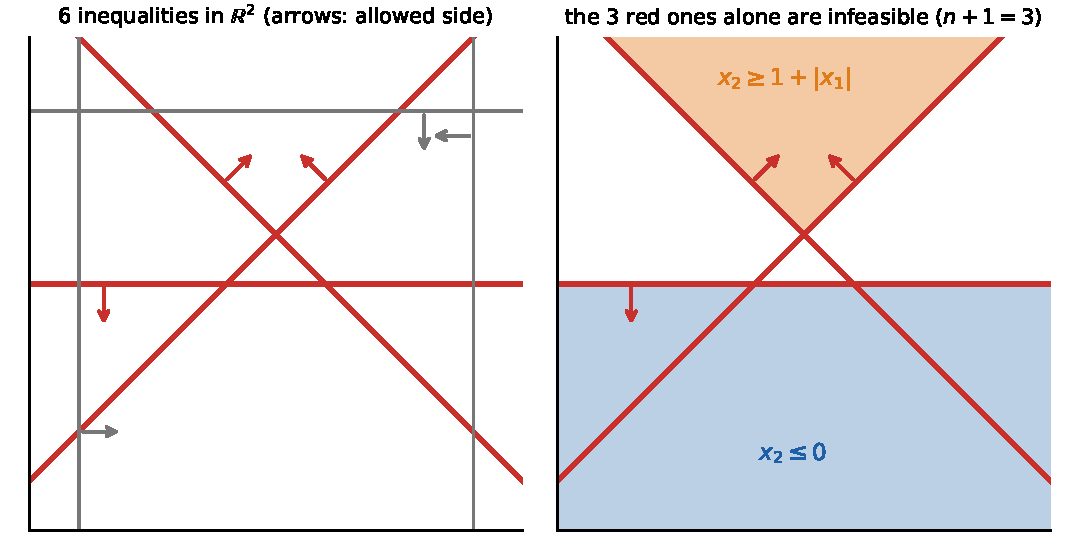
\includegraphics[width=.72\textwidth]{figures/p3_helly2d.pdf}\end{figure}
\begin{theorem}[Helly, for half-spaces]
If every $n+1$ members of a finite family of half-spaces in $\R^n$ have a common point, the whole family has a common point. (True for arbitrary convex sets as well.)
\end{theorem}
\begin{figure}[H]\centering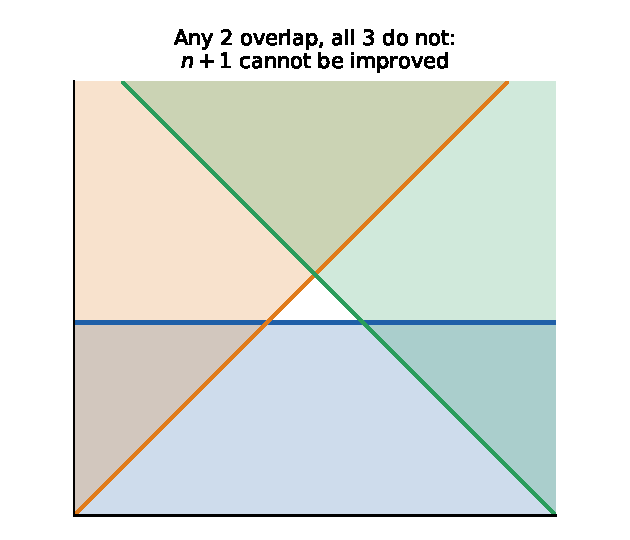
\includegraphics[width=.36\textwidth]{figures/g_tight.pdf}\end{figure}
\noindent The number $n+1$ is best possible: $x_j\ge1$ ($j\le n$) together with $\sum_jx_j\le n-1$ are jointly infeasible, yet every $n$ of them are feasible.

\begin{pitfall}
The bound counts \emph{equality rows of the dual}, not primal constraints. If the dual has redundant rows the true bound is the rank, which can be smaller, never larger. Also, ``at most $n+1$'' says nothing about \emph{which} subsystem: different vertices of the certificate polyhedron give different infeasible subsystems.
\end{pitfall}

\paragraph{Practical note.} When testing feasibility numerically, solve the phase-1 problem $\min t$ rather than passing a zero objective and trusting a status flag: the phase-1 LP is always feasible, its optimum quantifies the violation, and its dual solution \emph{is} the Farkas certificate.

\section{Self-test questions}
\begin{exercise} Write the dual of \ $\max\ 2x_1+x_2$ \ s.t.\ $x_1+x_2\le4$, \ $x_1-x_2\ge-2$, \ $x_1\ge0$, $x_2$ free.\end{exercise}
\begin{exercise} The primal is unbounded. What can the dual be? The dual is infeasible. What can the primal be?\end{exercise}
\begin{exercise} For $\max3x_1+2x_2$ s.t.\ $x_1+x_2\le4$, $x_1+3x_2\le9$, $x_1\le3$, $x\ge0$, use complementary slackness to verify that $x=(3,1)$ is optimal and find the dual solution.\end{exercise}
\begin{exercise} Prove Gordan's theorem: exactly one of ``$\exists x:Ax<0$'' and ``$\exists p\ge0,\ p\ne0,\ A\T p=0$'' holds.\end{exercise}
\begin{exercise} A system $Ax=b$, $x\ge0$ with $50$ equations and $1000$ unknowns is feasible. Show it has a solution with at most $50$ nonzero entries.\end{exercise}
\begin{exercise} Forty half-planes in $\R^2$ are such that every three have a common point. Must all forty have a common point?\end{exercise}
\begin{exercise} True or false: if $x$ and $p$ are feasible for a primal--dual pair and $x_j>0$ for some $j$ with $p\T A_j<c_j$, then $x$ is not optimal.\end{exercise}
\begin{exercise} In HW3 P3, suppose the 500 inequalities are in 600 variables. What does the theorem give?\end{exercise}

\subsection*{Answers}
\begin{enumerate}
\item Max problem: natural direction is $\le$. Row 1 ($\le$): $y_1\ge0$; row 2 ($\ge$): $y_2\le0$. $x_1\ge0$ gives a natural ($\ge$) dual constraint, $x_2$ free gives an equality:
$\min 4y_1-2y_2$ s.t.\ $y_1+y_2\ge2$, \ $y_1-y_2=1$, \ $y_1\ge0,\ y_2\le0$.
\item Dual must be infeasible. Primal is infeasible \emph{or} unbounded (it cannot have a finite optimum).
\item Dual: $\min4y_1+9y_2+3y_3$ s.t.\ $y_1+y_2+y_3\ge3$, $y_1+3y_2\ge2$, $y\ge0$. At $x=(3,1)$ row 2 is slack ($6<9$), so $y_2=0$; $x_1,x_2>0$ force $y_1+y_3=3$ and $y_1=2$, so $y=(2,0,1)\ge0$. Values: $11=8+0+3$. Optimal.
\item Not both: $0=(A\T p)\T x=p\T(Ax)<0$ since $p\ge0,\ p\neq0$ and $Ax<0$. At least one: $\max s$ s.t.\ $Ax+s\ones\le0$, $s\le1$ is feasible ($x=0,s=0$) and bounded. Its dual is $\min q$ s.t.\ $A\T p=0$, $\ones\T p+q=1$, $p,q\ge0$. If no $x$ has $Ax<0$ the primal optimum is $0$, so some dual-feasible point has $q=0$, i.e.\ $\ones\T p=1$: a nonzero $p\ge0$ with $A\T p=0$.
\item The feasible set is a nonempty standard-form polyhedron with $50$ equality rows; it has a BFS, which has at most $50$ positive entries.
\item Yes: Helly's theorem with $n=2$, $n+1=3$.
\item False. The pair violates complementary slackness, so $x$ and $p$ are not \emph{both} optimal, but the culprit may be $p$: any non-optimal dual-feasible $p$ has such a slack against an optimal $x$. To prove $x$ suboptimal you must show that \emph{no} dual-feasible $p$ is complementary to it.
\item An infeasible subsystem of at most $\min\{500,\,601\}=500$ inequalities: nothing. The result is only informative when $m>n+1$.
\end{enumerate}

\section{One-page cheat sheet}
\begin{center}\renewcommand{\arraystretch}{1.3}
\begin{tabular}{@{}>{\raggedright}p{.29\textwidth}p{.64\textwidth}@{}}\toprule
Dual of $\min c\T x$ & $\max p\T b$; rows $\ge/\le/=$ $\to$ $p_i\ge0/\le0/$free; vars $\ge0/\le0/$free $\to$ $p\T A_j\le/\ge/=c_j$\\
Lagrangian view & $g(p)=p\T b+\min_x(c-A\T p)\T x$; signs of $p$ make it a lower bound, dual constraints make it finite\\
Weak duality & $p\T b\le c\T x$. Unbounded primal $\Rightarrow$ infeasible dual\\
Strong duality & optimal solution on one side $\Rightarrow$ optimal on the other, equal values; no gap for LPs\\
Impossible combinations & finite/unbounded, finite/infeasible, unbounded/unbounded\\
Both infeasible & possible\\
Complementary slackness & $p_i(a_i\T x-b_i)=0$, $(c_j-p\T A_j)x_j=0$ $\iff$ feasible pair is optimal\\
Geometry of optimality & $c\in\operatorname{cone}\{a_i:i\text{ active at }x^\star\}$\\
Farkas & $Ax=b,x\ge0$ \ XOR \ $p\T A\ge0,\ p\T b<0$\\
Farkas (inequalities) & $Ax\le b$ \ XOR \ $p\ge0,\ A\T p=0,\ b\T p<0$\\
Gordan & $Ax<0$ \ XOR \ $p\ge0,\ p\neq0,\ A\T p=0$\\
HW3 P2 & $(Ax\ge0,x\ge0\Rightarrow x_1=0)\iff\exists p\ge0:\ p\T A\le0,\ p\T A_1<0$\\
Proving alternatives & easy direction: multiply and add; hard direction: LP + dual + strong duality\\
Strict inequality trick & homogeneous system: $p\T A_1<0\iff$ (after scaling) $p\T A_1\le-1$\\
BFS sparsity & $\{Mx=d,x\ge0\}$ nonempty $\Rightarrow$ solution with $\le\operatorname{rank}M$ nonzeros; optimal BFS exists if an optimum exists\\
HW3 P3 & infeasible $Ax\le b$ in $\R^n$ $\Rightarrow$ infeasible subsystem of $\le n+1$ rows (support of a dual vertex); tight\\
Helly / Carath\'eodory & every $n+1$ intersect $\Rightarrow$ all intersect; hull points need $\le n+1$ generators\\
Phase-1 LP & $\min t$ s.t.\ $a_i\T x-t\le b_i$; \ $t^\star>0\iff$ infeasible; dual optimum is the certificate\\ \bottomrule
\end{tabular}\end{center}

\bigskip\noindent\textbf{Further reading.} Bertsimas \& Tsitsiklis, \emph{Introduction to Linear Optimization}, Ch.~2 (BFS, \S2.2--2.6) and Ch.~4 (duality, \S4.1--4.7; Farkas in \S4.6). Boyd \& Vandenberghe, \emph{Convex Optimization}, \S5.1--5.2 (Lagrange dual), \S5.5 (complementary slackness/KKT), \S5.8 (theorems of alternatives).
\end{document}
